\section{Orbite de la Terre (4 points)}

La Terre tourne autour du Soleil à une distance moyenne d'environ 150 millions de kilomètres suivant une période de \num{365.25} jours. On considère que le mouvement de la Terre autour du Soleil est circulaire.

\begin{center}
	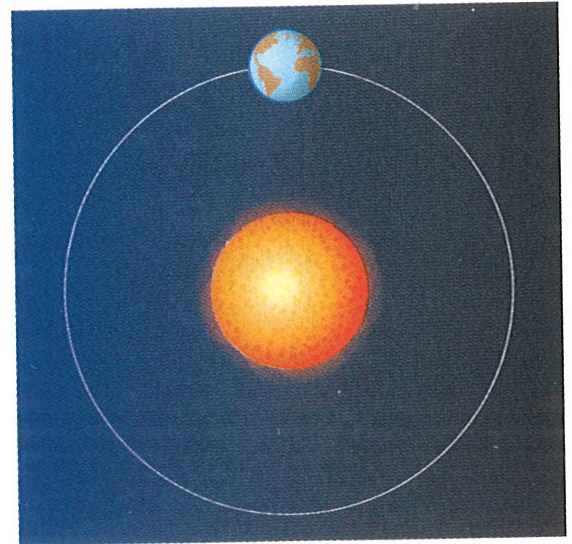
\includegraphics[scale=0.5]{terre}
\end{center}

\begin{questions}
	\question[2] Quelle est la distance parcourue par la Terre autour du Soleil pendant une année ?
	\fillwithdottedlines{3cm}
	
	\question[2] Calculer la vitesse de rotation de la Terre en km/h puis en km/s.
	\fillwithdottedlines{3cm}
\end{questions}